\normaltrue \difficilefalse \tdifficilefalse
\correctionfalse
%\UPSTIidClasse{11} % 11 sup, 12 spé
%\newcommand{\UPSTIidClasse}{11}

\exer{Système éclipse $\star$ \label{C2:04:65}}
% Banque PT SI A 2009
\setcounter{question}{0}\UPSTIcompetence[2]{C2-04}
\index{Compétence C2-04}
\index{Correcteur}
\index{Correcteur proportionnel}
\index{Système éclipse}


\ifcorrection
\else
\marginnote{\textbf{Pas de corrigé pour cet exercice.}}
\fi

\ifprof
\else 

Le schéma-blocs sous la forme suivante avec un gain unitaire pour le capteur
de vitesse.

\begin{center}
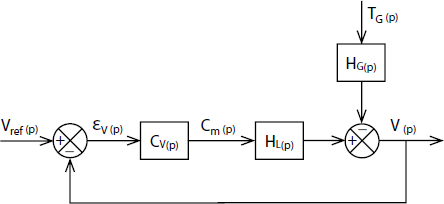
\includegraphics[width=\linewidth]{65_01}
\end{center}

$H_L(p)=\dfrac{K_L}{1+\tau_L p}$ et $H_G(p)=\dfrac{K_G}{1+\tau_G p}$  avec $\tau_G=\tau_L = \SI{20}{ms}$, $K_L = \SI{1e-3}{N^{-1}s^{-1}}$ et $K_G = \SI{2e-5}{mN^{-1}s^{-1}}$.


Le cahier des charges donne les valeurs des critères d'appréciation adoptés :
\begin{itemize}
\item la précision : en régime permanent à vitesse constante, soit $\varepsilon_S=0$ et à accélération constante, soit $\varepsilon_T=0$; $\varepsilon_S$ désigne l'erreur statique de position et $\varepsilon_T$ l'erreur statique de vitesse ou erreur de traînage;
\item la rapidité : le temps de réponse à \SI{5}{\%} tel que : $t_{\text{R}\SI{5}{\%}}\leq \SI{1}{s}$;
\item la stabilité : marge de phase $\geq \SI{45}{\degres}$ et marge de gain $\geq \SI{10}{dB}$.
\end{itemize}

On choisit tout d'abord une correction proportionnelle telle que $C_V(p)=K_P$.
\fi

\question{Le cahier des charges est-il respecté en termes de précision, rapidité et stabilité ?}
\ifprof
\else 
\fi

\question{Peut-on choisir une valeur de $K_P$ qui puisse assurer le respect complet du cahier des charges ?}
\ifprof
\else 
\fi

\question{Le système est-il robuste à une perturbation en échelon ?}
\ifprof
\else 
\fi

\ifprof
\else

\noindent\footnotesize
% \fbox{\parbox{.9\linewidth}{
% Éléments de corrigé : 
% \begin{enumerate}
  % \item $\varepsilon_{\text{con \%}} = \dfrac{1}{1+K_PK_m K_{\text{pom}} K_{\text{cap}} }$;
  % \item $K_P > 19$;
  % \item $\varepsilon_{\text{pert}} = \Delta Q_e \dfrac{K_f}{1+K_{\text{cap}}K_PK_mK_{\text{pom}}}$;
  % \item $K_P > 2,19$.
  % \item $K_P < 0,125$. Il est impossible de vérifier les trois conditions avec un correcteur proportionnel.
% \end{enumerate}}}
\normalsize

\begin{flushright}
\footnotesize{Corrigé  voir \ref{C2:04:65}.}
\end{flushright}%
\fi